\documentclass[tikz,border=10pt]{standalone}
\begin{document}
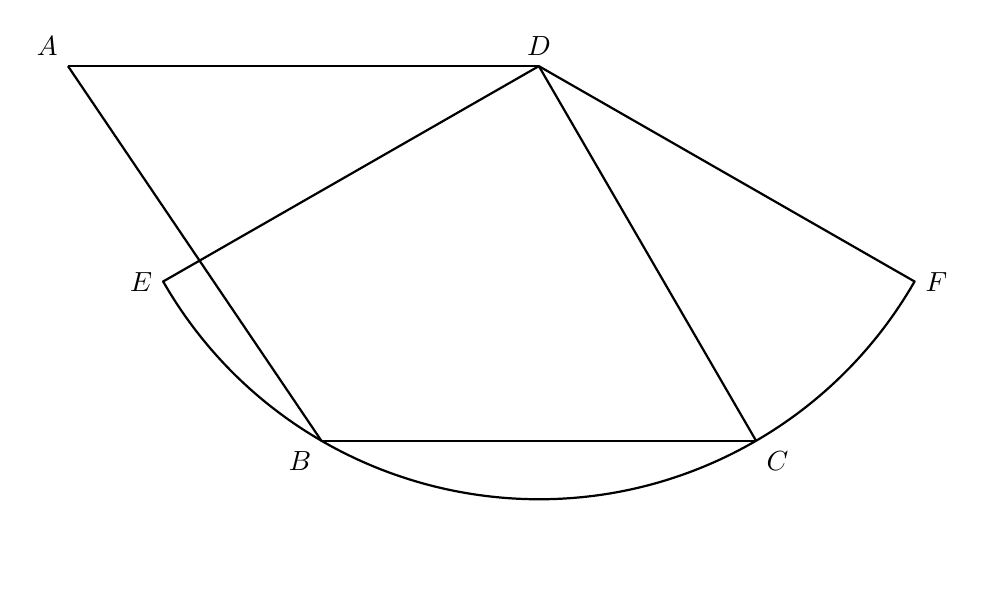
\begin{tikzpicture}[scale=1, line width=0.8pt]
\coordinate (A) at (1.36,-1.34);
\coordinate (D) at (7.34,-1.34);
\coordinate (E) at (2.56,-4.08);
\coordinate (F) at (12.12,-4.08);
\coordinate (B) at (4.58,-6.10);
\coordinate (C) at (10.10,-6.10);

\draw (A) -- (D);
\draw (A) -- (B);
\draw (D) -- (E);
\draw (D) -- (F);
\draw (D) -- (C);
\draw (B) -- (C);
\draw[shift={(D)}] (209.8:5.5) arc[start angle=209.8, end angle=330.2, radius=5.5];

\node[above left] at (A) {$A$};
\node[above] at (D) {$D$};
\node[left] at (E) {$E$};
\node[right] at (F) {$F$};
\node[below left] at (B) {$B$};
\node[below right] at (C) {$C$};
\end{tikzpicture}
\end{document}
